\documentclass{TDP003mall}
\usepackage{titlesec}
\usepackage{graphicx}
\definecolor{terminalgreen}{HTML}{8AE234}

\newcommand{\version}{Version 0.1}
\author{Eric Jönsson, \url{erijo137@student.liu.se}\\
  Ida Bergquist, \url{idabe112@student.liu.se}}
\title{Systemdokumentation}
\date{2018-10-16}
\rhead{Ida Bergquist\\
Eric Jönsson}



\begin{document}
\projectpage
\tableofcontents
\newpage
\section{Revisionshistorik}
\begin{table}[!h]
\begin{tabularx}{\linewidth}{|l|X|l|}
\hline
\textbf{Ver.} & \textbf{Revisionsbeskrivning} & \textbf{Datum} \\\hline
0.1 & Skapade systemdokumentationen & 181016 \\\hline
\end{tabularx}
\end{table}

\section{Overview}
\begin{figure}[h!]
    \centering
    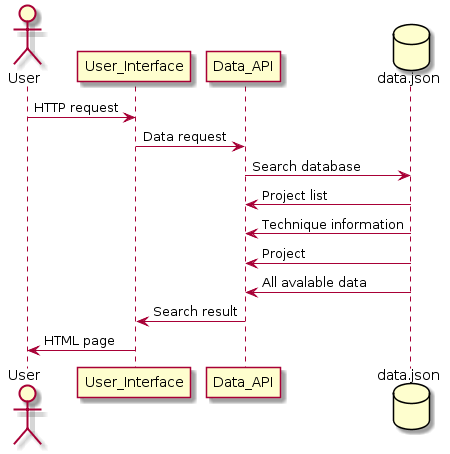
\includegraphics[width=10cm]{sevenskdiagram.png}
    \caption{Simplified view of the portfolio}
    \label{sekvensdiagram}
\end{figure}

\section{Design}
\subsection{Data API}
All functions are defined in a seperate document called module\_documentation.pdf.
\subsection{User interface}
\begin{figure}[h!]
    \centering
    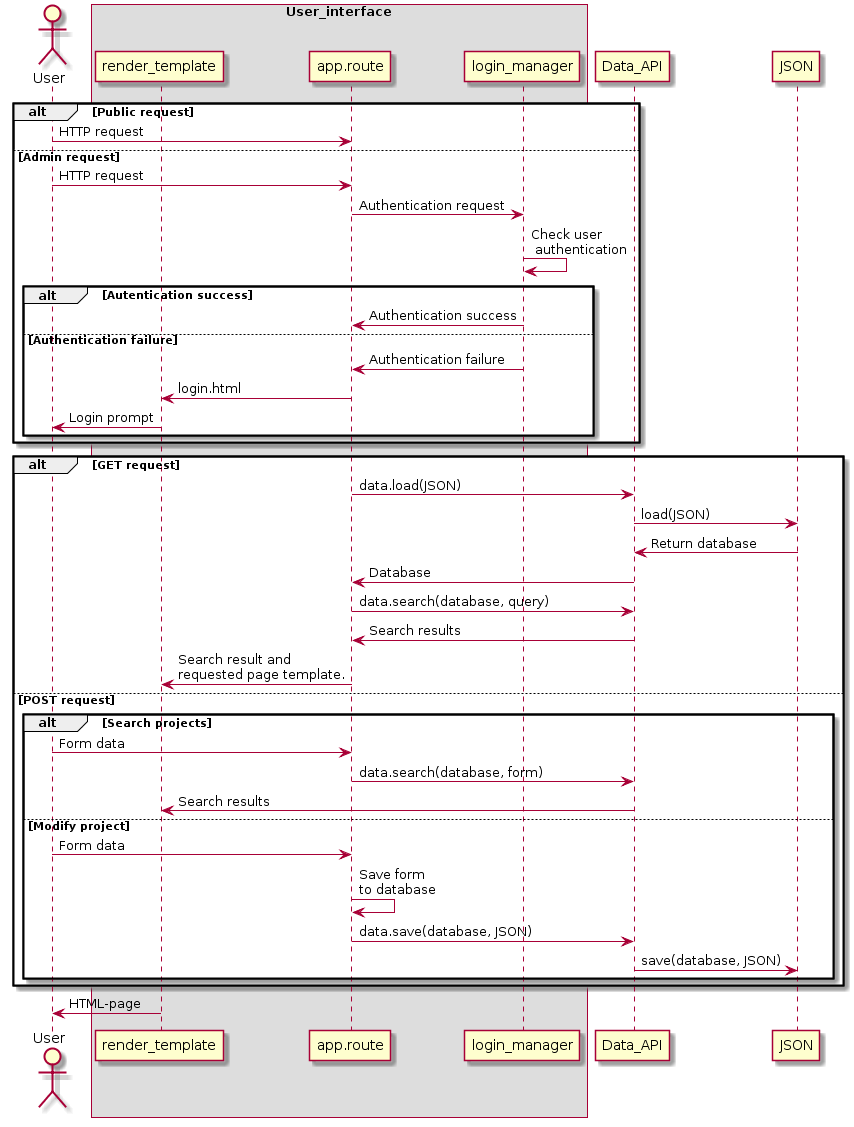
\includegraphics[width=\linewidth]{sekvensdiagram2-3.png}
    \caption{The inner workings of the user interface}
    \label{sekvensdiagram2}
\end{figure}
All functions
\section{Errors and errorlogs}
\subsection{Logs}
When the project is running logs are printed out directly to the terminal.
No file logging is performed.

\subsection{Tests}
The Data API is built to handle the unit tests present at: \href{https://gitlab.ida.liu.se/filst04/tdp003-2018-database-tests}{Database Tests}. These
tests can be cloned into a suitable folder on a local computer and ran to
verify that the Data API works as intended. Please note that in order to run
the tests, the data.py file from the project has to be present in the
same folder as the data\_test.py file from the database test repo.
To run the tests simply execute data\_test.py within your terminal.

No specific tests are executed on the front end itself, however one might
concievably want to write some on one's own.

\end{document}
